
% Miranda's veil chapter ----------------------------------------------
\chapter*{Miranda's veil}
\addcontentsline{toc}{chapter}{Miranda's veil}

\begin{flushright}
\parbox{0.8\textwidth}{
\emph{Under all that we think, lives all we believe, like the ultimate veil of our spirits. \\
\hspace*{\fill}{\textperiodcentered \textperiodcentered \textperiodcentered \hspace*{0.2em} Antonio Machado} } }
\end{flushright}

\noindent
Miranda's veil is chess variant which is played on 16 x 16 board,
with light yellow and dark violet fields and light pink and dark
gray-violet pieces. In algebraic notation, columns are enumerated
from 'a' to 'p', and rows are enumerated from '1' to '16'. A new
piece is introduced, Wave.

\clearpage % ..........................................................

\section*{Wave}
\addcontentsline{toc}{section}{Wave}

\noindent
\begin{wrapfigure}[12]{l}{0.4\textwidth}
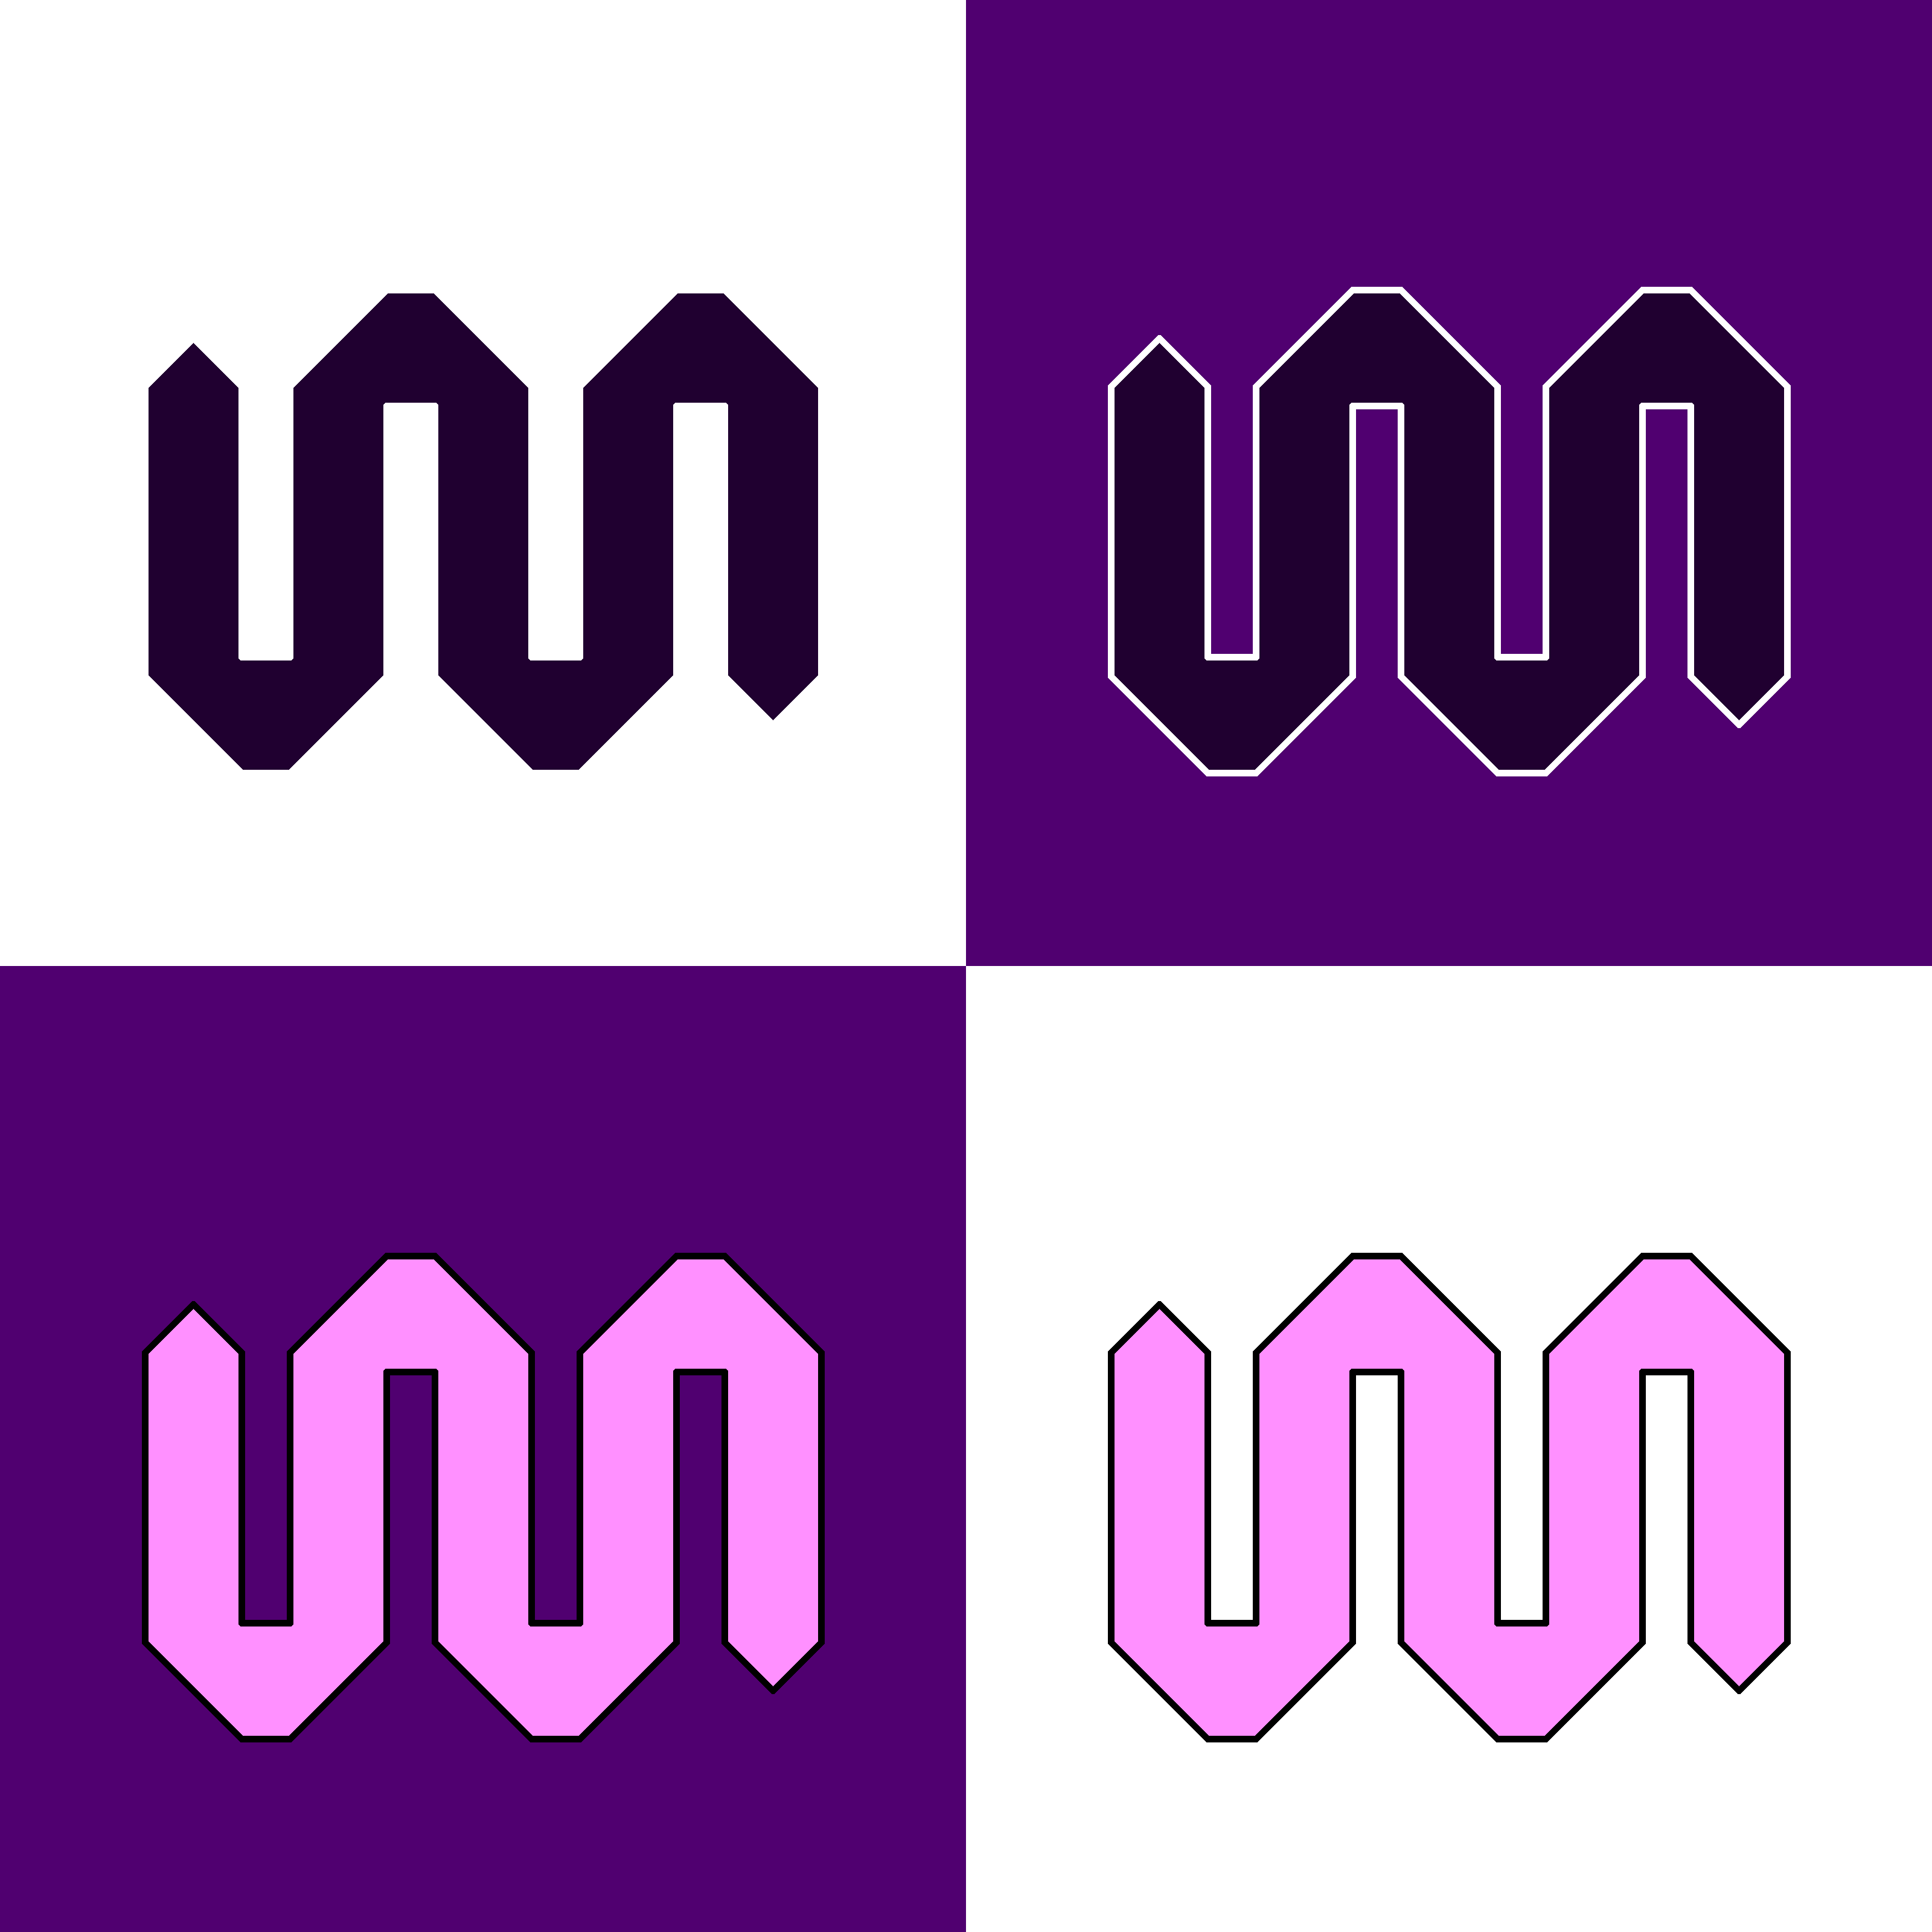
\includegraphics[width=0.4\textwidth, keepaspectratio=true]{pieces/10_wave.png}
\caption{Wave}
\label{fig:wave}
% % \centering
\end{wrapfigure}
Wave is passive piece, it has to be activated before it can move.
Activation is done in the same way as with Pyramid. Own piece
has to capture field at which Wave is located before Wave can
move.

After activation Wave moves like Queen. Pawn can activate Wave
not just at its' capture-fields, but also on its' step-fields.
Wave is not blocked by any piece, it can continue its' movement
freely, as if there are no pieces on board at all.

Wave cannot capture any piece. Consequenly, Wave cannot check
opponent's King, and hence can't participate in a checkmate.

Wave can activate any own piece, except King. Wave can also
activate opponent's Wave.

In algebraic notation, symbol for Wave is 'W'.

\subsection*{Activation}
\addcontentsline{toc}{subsection}{Activation}

For the next few examples I'll use the same setup, shown on next
page, with Pegasus making 5-step move before activating Wave. That
is momentum Wave will be receiving with activation.

\clearpage % ..........................................................

\noindent
% \begin{figure}[t]
\begin{figure}[h]
\includegraphics[width=1.0\textwidth, keepaspectratio=true]{examples/10_move_wave_init.png}
\caption{Wave activation}
\label{fig:wave_activation}
% \centering
\end{figure}

As before, activation of Wave is done by full move to left by Pegasus,
shown in red. Note that Pegasus, just as any other piece, cannot move
past Wave, except another Wave, own or opponent's, shown in grey.

\clearpage % ..........................................................

Unlike any
other piece, Wave does not spend received momentum moving, it can
move past momentum limit, in this case for more than just 5 fields.
Momentum carried by Wave is in entirety transferred to piece
activated by said Wave (or lost if no piece is activated).

\clearpage % ..........................................................

\subsection*{Cascading}
\addcontentsline{toc}{subsection}{Cascading}

\clearpage % ..........................................................

\section*{Initial setup}
\addcontentsline{toc}{section}{Initial setup}

Initial setup can be seen in image below:

\noindent
% \begin{figure}[t]
\begin{figure}[h]
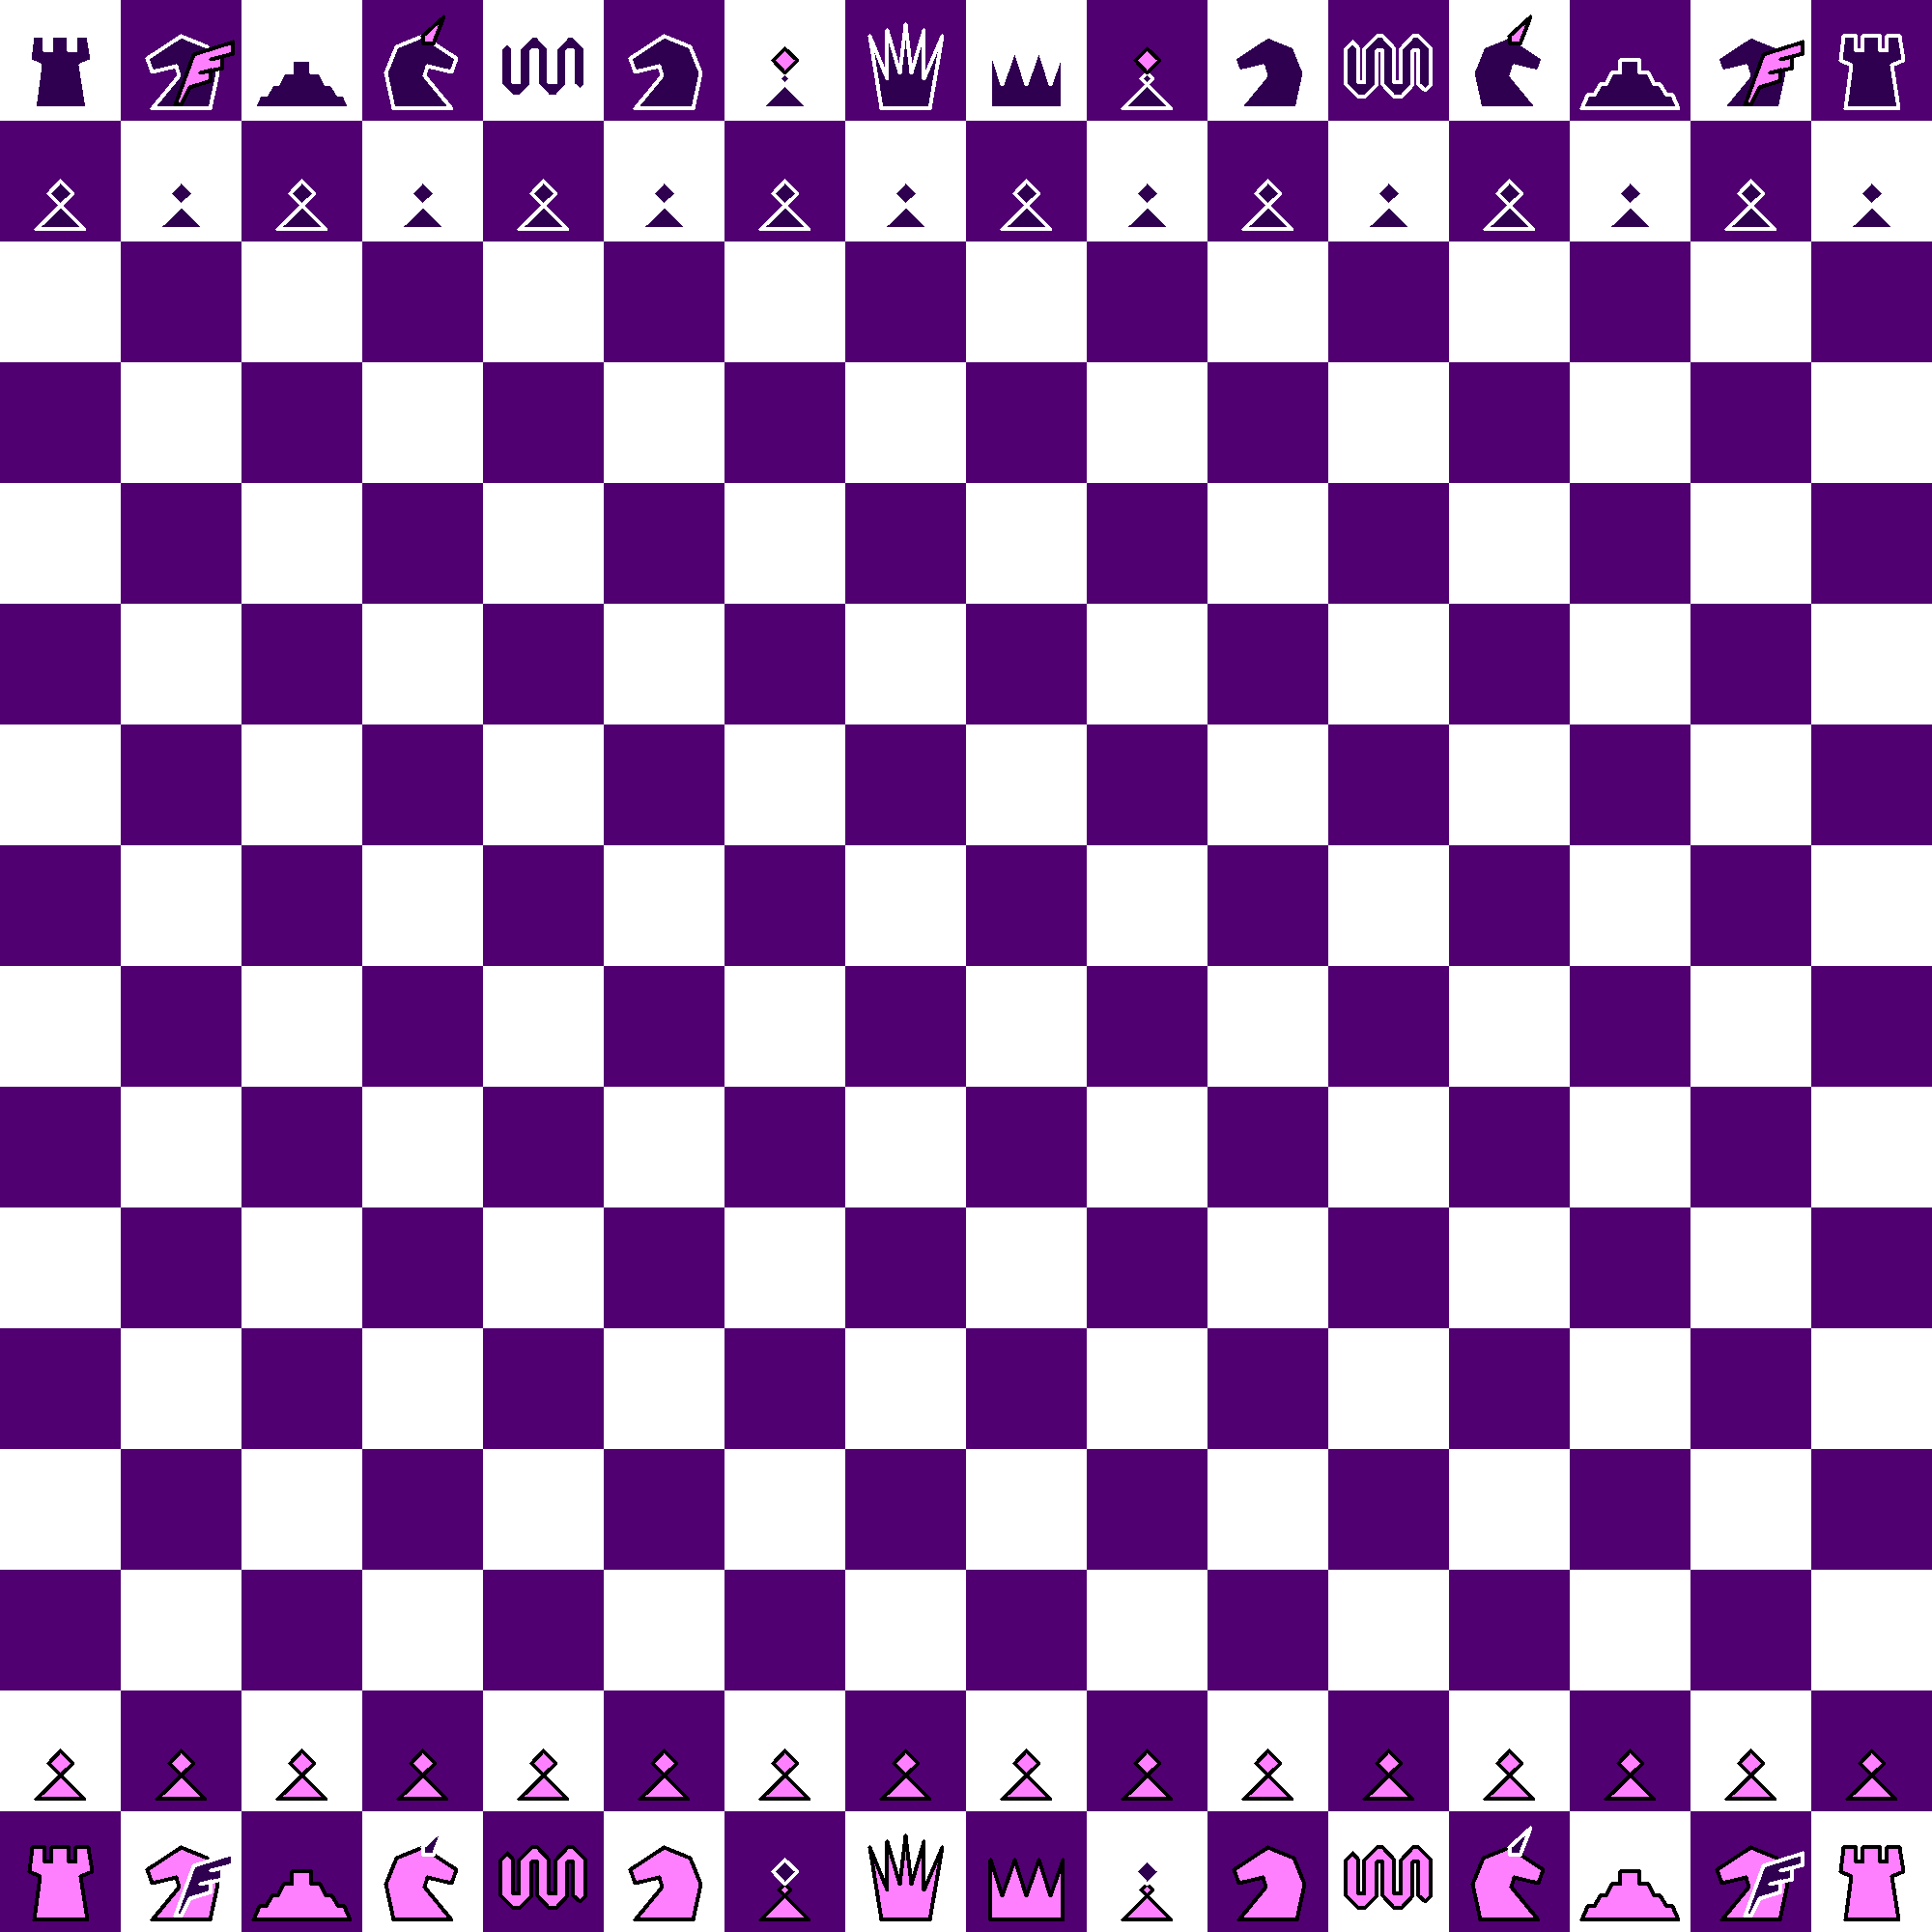
\includegraphics[width=1.0\textwidth, keepaspectratio=true]{boards/10_miranda_s_veil.png}
\caption{Miranda's veil board}
\label{fig:miranda_s_veil}
% \centering
\end{figure}

\clearpage % ..........................................................
% ---------------------------------------------- Miranda's veil chapter
